\chapter{A survey of Cognitive Architectures}
\label{The_nature_of_cognition}
\newcommand{\soar}{\small SOAR\ }
\newcommand{\actr}{\small ACT-R\ }
The quest to understand the working of the human mind has spanned
many centuries starting with Plato when he asked, as in the words of
Noam Chomsky citing Bertrand Russell, ``{\bf How is it that human beings,
whose contacts with the world are brief, personal and limited, are
nevertheless able to know as much as they do?}'' \cite{Bogdan:1993aa}


Cognitive science brings together the varied disciplines of
psychology, neuroscience, computer science, linguistics and philosophy
in an attempt to answer the above question, using information
processing as a means to emulate the human mind. Psychology,
especially cognitive psychology, contributes theories on cognitive
capacities, information processing capabilities of , and so forth.
Perhaps most importantly, it theorizes about the overall picture of
the human mind. Neuroscience, the study of the brain and nervous
system, provides a frame of reference against which theories developed
in cognitive science can be validated since it deals with the brain at
the lowest level.
% 
% Secondly, it provides knowledge for developing an alternative
% architecture of the mind. -- I was reffering to the connectionist
% architectures.
%
Computer science contributes knowledge representation, which is used
to develop theories to represent the way knowledge is stored,
artificial intelligence, which is used to analyse and create methods
for problem solving, and the theory of computation, which is used as a
means to understand foundational limits on cognition as
information processing.

The objective of this chapter is three-fold.  Firstly it aims to
provide a very brief introduction to the human cognitive architecture
from both the cognitivist and emergent
\cite{DBLP:journals/tec/VernonMS07} perspectives.  Secondly it
discusses cognitive architecture in general.  Finally it goes on to
compare some currently and widely used cognitive architectures.

\section{The nature of cognition}
\label{nature_Of_Cognition}
Any attempt to deal with the architecture of cognition has to answer
the following questions.

\begin{itemize}
\item \emph{What is knowledge and how can it be categorized?}  Since the aim
  of cognitive science is to understand the working of the human mind
  it is essential the nature of knowledge is understood because human
  beings function by processing information. Therefore it is
  imperative that we understand what knowledge is and the different
  forms of knowledge that are available.

  Although the nature of knowledge has been studied over many
  millennia we are still not certain of its characteristics. Here I
  will briefly describe what Brachman and Levesque in
  \cite{brachman-levesque:2004a} have to say about the nature of knowledge.
  They describe as one perspective of knowledge as a function that
  maps a knower to a proposition. A proposition is a statement that
  determines the truth value of the belief of the knower. But they
  also acknowledge that not all knowledge is of this form, for example

\item \emph{How is knowledge acquired, represented and utilized?} When
  solving problems the human mind has the ability to retrieve and
  apply previously stored knowledge to the problem; for example,
  consider solving a calculus based integration problem.  We are able
  to retrieve standard representations of the forms of equations and
  apply them to the problem to simplify it and solve it.   Issues
    of knowledge retrieval and application are central to
  understanding cognition.

\item How do various processes act on this knowledge and how do they
  achieve the effect they intend to achieve?  These two areas are
  significant because of their relationship to the techniques of
  deduction and inference that we use to solve problems on an everyday
  basis, inferences as simple and routine as when we diagnose a faulty
  light, or the more complex techniques we use when solving a
  crossword puzzle.

\item How can these processes and structures be manifested in the real
  world? \textsc{Waiting for prof response}
\end{itemize}


These questions provide us with a very general framework of the
results to be provided by cognitive
science. Newell~\cite{,Newell1980135} describes the study of the
working of the mind as a problem of satisfying the ``Conjunction of
constraints on the nature of mind like systems.'' He describes the
characteristics of what is to be expected of any theory that claims to
propose a model of human cognition. Newell mentions that this list is
not comprehensive, but in the view of Anderson and Lebiere
\cite{CambridgeJournals:207162} it can used to provide a broad
framework against which all theories that claim to explain the human
mind can be tested.
 
These criteria, listed below, have been discussed in the
literature~\cite{CambridgeJournals:207162,Newell:1990aa}. The purpose
of listing these criteria below is to explain as to what the study of
the mind would require.

\begin{itemize} 


\item Behave flexibly as a function of the environment: At first
glance this statement may seem frivolous, as it seems to imply that
human cognition functions in a haphazard manner. But Newell did make it clear
that he was referring to the view that a cognitive system can be
viewed as an instance of a universal computer, specifically a turing
machine, despite its occasional failings and lack of infinite
memory. He further explains that this view does not indicate the
inablity to perform special operations, for example, vision. He
explains that like computers with special processing units the
cognitive system can be made up of special purpose systems that
specialize in a certain task. As an example consider the example of
chemist they are able to perform congnitive tasks that are relates to
their field and they are also able to drive their car. 


\item Operate in real time: A system that models cognition should be
able to explain the reason as to how we are able to perform cognitive
tasks at the speed humans do. This criteria is important because if a
system is not able to explain it could lead us to wrong assumptions
about how humans think.


\item Exhibit rational adapative behaviour: It must be able to explain
this because humans perform computations and those computations, as in the words of
Newell\cite{Newell:1990aa}, are for ``the service of goals and
rationally related to obtaining things that let the organism survive
and propagate.''

\item Display dynamic behaviour: Humans operate in an
environment that is ever changing. They draw in this
information from their environment and act on it appropriately. For
example, if you are driving a car and at that moment a deer decides
to sprint in front of the car, you would hit the brakes. 


\item Integrate diverse knowledge: Humans acquire knowledge from
diverse sources and are able to integrate them. For example consider a
computer programmer working in the banking industry. He can go to
school to obtain knowledge of the working of the finance industry. He
can use this knowledge along with his knowledge of computers science
to write programs for the industry. Here we see that our fictitious
programmer integrating knowledge, unlike expert systems where
knowledge is vertical and cannot be integrated as easily.

\item Exhibits a sense of consciousness: Newell could not point out to
  the direct relation between consciousness and human cognition but he
  did mention it as one of the criteria in his tests of human
  cognition. One interpretation of
  this~\cite{CambridgeJournals:207162} is that Newell was asking us to
  pick out criteria for this test and the authors of that paper point
  towards using sections from \cite{Cohen:1996aa}

\item Learning from the environment: This point should be self
evident, we gain new knowledge from the world around us. But then
the type of learning itself should be based on whether it can learn based on
semantic memory, skill, priming and conditioning.

\item Arise through evolution: It is understood that the algorithms we
use today are those that have arisen naturally over a period of time,
hence any cognitive architecture should be able to learn and improve
the algorithms through an process of constant improvement.

\item Use of Natural language: Any theory that claims to decipher human
cognition must be able to explain as to how we are able to comprehend
what we listen, understand what we speak because this is a function
that is core to the way we communicate with each other.

\item Be realizable with in the brain: This point is critical because
it serves as proof that a given theory is congruous with actual
computations in the brain.

\end{itemize}
\section{Approaches towards explaining cognition}
    There are many theories on the nature of cognition, each
    taking a position on what constitutes cognitive functions and how
    they are carried out. But these approches can be bifurcated into
    approaches that adhere to the \emph{cognitivist
    approach}~\cite{DBLP:journals/tec/VernonMS07}, theories
    that view cognition as information processes manipulating symbols,
    and those that stick to the \emph{emergent approach}, theories
    that treat cognition as a process where models reflect the
    processes of cognition by reorganizing themselves to 


    The goal of objective of this section is to explore these points
    of view and conclude by bringing out differences between these
    disparate points of view, after which we examine a number of
    cognitive architectures in detail.
\subsection{The Cognitivist view}
     
     The cognitivist perspective views human cognition as a set of
     information processes working over a set of representations that
     point to the actual knowledge which may be stored else where,
     vis-\'{a}-vis symbols. These information processes are said to be
     purposeful, contentful, representational and can be described
     formally\cite{103009}. Knowledge derived from these computations
     can be stored and used later to improve the reasoning of the
     system. The cognitivist views the function of perception is to
     generate an appropriate representation of the the world around
     the system which the system uses to reason
     \cite{DBLP:journals/tec/VernonMS07}.

     The task of building models in cognitivist system is generally
     done by a programmer. Which is good in a way that these
     representations and structures can be viewed and interpreted by
     humans. But it may also ``bias the system'' and constrain it to an
     idealized cognitive environment. As a result this cause
     problems when the system does have to stray away from this
     requirements, this gap between perception, which is in
     interpretation of reality, and actual reality begin to
     widen. This would then have to be filled in with more programmer
     knowledge to close this ``semantic
     gap''\cite{DBLP:journals/tec/VernonMS07}. 
     
\subsection{The Connectionist approach}


     Until the 1980s the cognitivist viewpoint was the primary means
     of explaining the nature of human cognition. Interest in
     self-organizing systems led to an area of research that advocated
     the view that human cognition is made up of smaller units that
     rearrange themselves as the system acquires a skill or recognizes
     a change in its environment. This approach to understanding is
     known as the \emph{emergent approach}
     \cite{DBLP:journals/tec/VernonMS07}.
     
     Although there are multiple methods are used to in the area of
     emergent systems, I will describe only connectionist view
     point. Connectionism defined by Medler in \cite{Medler98abrief}
     as ``a theory of information that uses parallel processing of
     sub-symbols, using statistical properties instead of logical
     rules to transform information'' rather than rules as used in
     classical cognitivist systems.

     The basic feature in a connectionist system is a connectionist
     network. A connectionist network is made up of a number of simple
     computational units that communicate with each other with via
     connections. These connections are capable of carrying only
     simple information.
     
     The computational units in a connectionist system are arranged in
     a number of hierarchical layers. These layers are the input
     layer, the hidden layer, the output layer. The input layer These
     networks can be arranged into two basic configurations namely
     \emph{feed forward} networks and \emph{recurrent} networks.

     Feed forward networks(Fig \ref{ASCA_AFFN}) are those networks in
     which information flows in one direction only, that is from the
     input layer to the hidden layers(if they exist) and then to the
     output layer. Recurrent networks are those networks that have
     loops and hence backward connections

     \begin{figure}[htp]
     \centering
     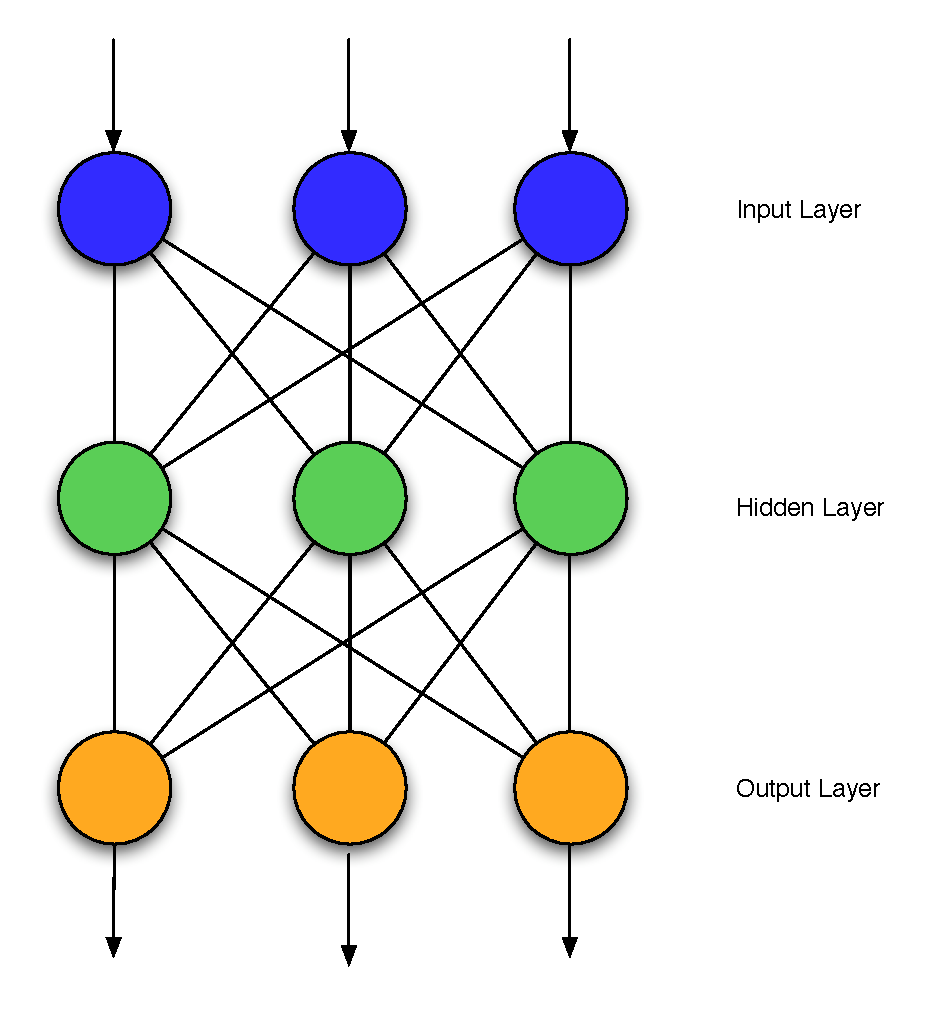
\includegraphics[width=80mm]{FeedForwardNetwork.eps}
     \caption{A feed forward network}
     \label{ASCA_AFFN}
     \end{figure}
     
     Connectionist models learn by adjusting the weights on the
     individual computational units. This implies that learning in
     connectionist models can be viewed more as a skill building
     exercise, rather than an exercise in knowledge acquistion as in
     the case of the congitivist approaches
     \cite{DBLP:journals/tec/VernonMS07}.
     
     The main attraction of connectionism is that it provides a means
     to provide neural plausibility\cite{103009} to theories of
     cognitive science because of its ability to simulate the
     massively parallel processing in the brain and also its ability
     to learn by adjusting weights. It is also attractive because it
     provides cognitive plausbility by allowing problems to be studied
     using simpler mechanisms, they could help in studying the
     processes underlying the processes of pattern-recognition and
     memory retrival and the ability to apply soft constraints when
     representing schematic knowledge.

     Despite these attractions connectionist models find it difficult
     to explain the ability of the human mind to to integrate diverse
     knowledge from various sources, the ability to use pre-existing
     knowledge and the ability to respond with in the time constraints
     that humans do.

     
\section{Cognitive Architectures}
% Talk about the need for cognitive architectures
Early work in psychology focused on proving micro theories. Although
each of these microtheories explained their individual specializations
well no one attempted to integrate these to provide an complete
picture of human cognition)\cite{citeulike:4408336}. For example
(TODO:Check a theory about memory and then about productions). Newell
called for scientists in the area towards providing a complete
framework of human cognition and proving theories within it.
\cite{Newell:1990aa, citeulike:4408336}

Therefore based on this we can define a cognitive architecture as

\begin{quote}
A framework that provides an interpretation of the working of
human cognition within which theories related to various aspects of
cognition can be validated based on that interpretation.
\end{quote}

% Explain the above definition more clearly
As mentioned earlier the most basic view of human cognition is that of
solving a constraint solving problem\cite{Newell:1990aa}. As of now
cognitive science is a developing field and there can be numerous ways
as to how these constraints can be interpreted and solved by
researchers. In such a case, that researcher is providing us with an
interpretation of what he or she believes how the mind works.

% SUN: He is explaining what the concept of architecture by providing
% an analogy to what architecture provides and things that can be
% moved around inside.
An cognitive architecture provides us with an invariant environment
where we can perform detailed modeling that helps us in understanding
the processes, structures and the organization between these
structures in the brain\cite{journals/jetai/Sun07}.
 

% List out the uses of cognitive architectures
Sun\cite{journals/jetai/Sun07} lists out the significance of the study
of cognitive architectures as follows
\begin{itemize}
\item Provide a means of understanding cognition.
\item They provide a foundation to build intelligent systems that are
  cognitively realistic.
\end{itemize}

Moving on from here we will discuss the criteria for comparing
cognitive architecture and we will also look at some sample cognitive
architectures.

% Define and explain what is needed from a cognitive architecture.
\section{Survey of cognitive architectures}

This section I will describe a number of popular cognitive
architectures that are currently in use. I will later compare them
based on a number of criteria that reflect the functions that a
congitive architecture is supposed to perform.

% General template
% Describe architecure
%   Knowledge representation, 
%      short term memory, long term memory, Goals,
%   Mechanics of cognition
%      Means of planning, Learning
%   Abilities of perception
%      Auditory, Visual

\subsection{ACT-R}

\begin{figure}[htp]
  \centering
  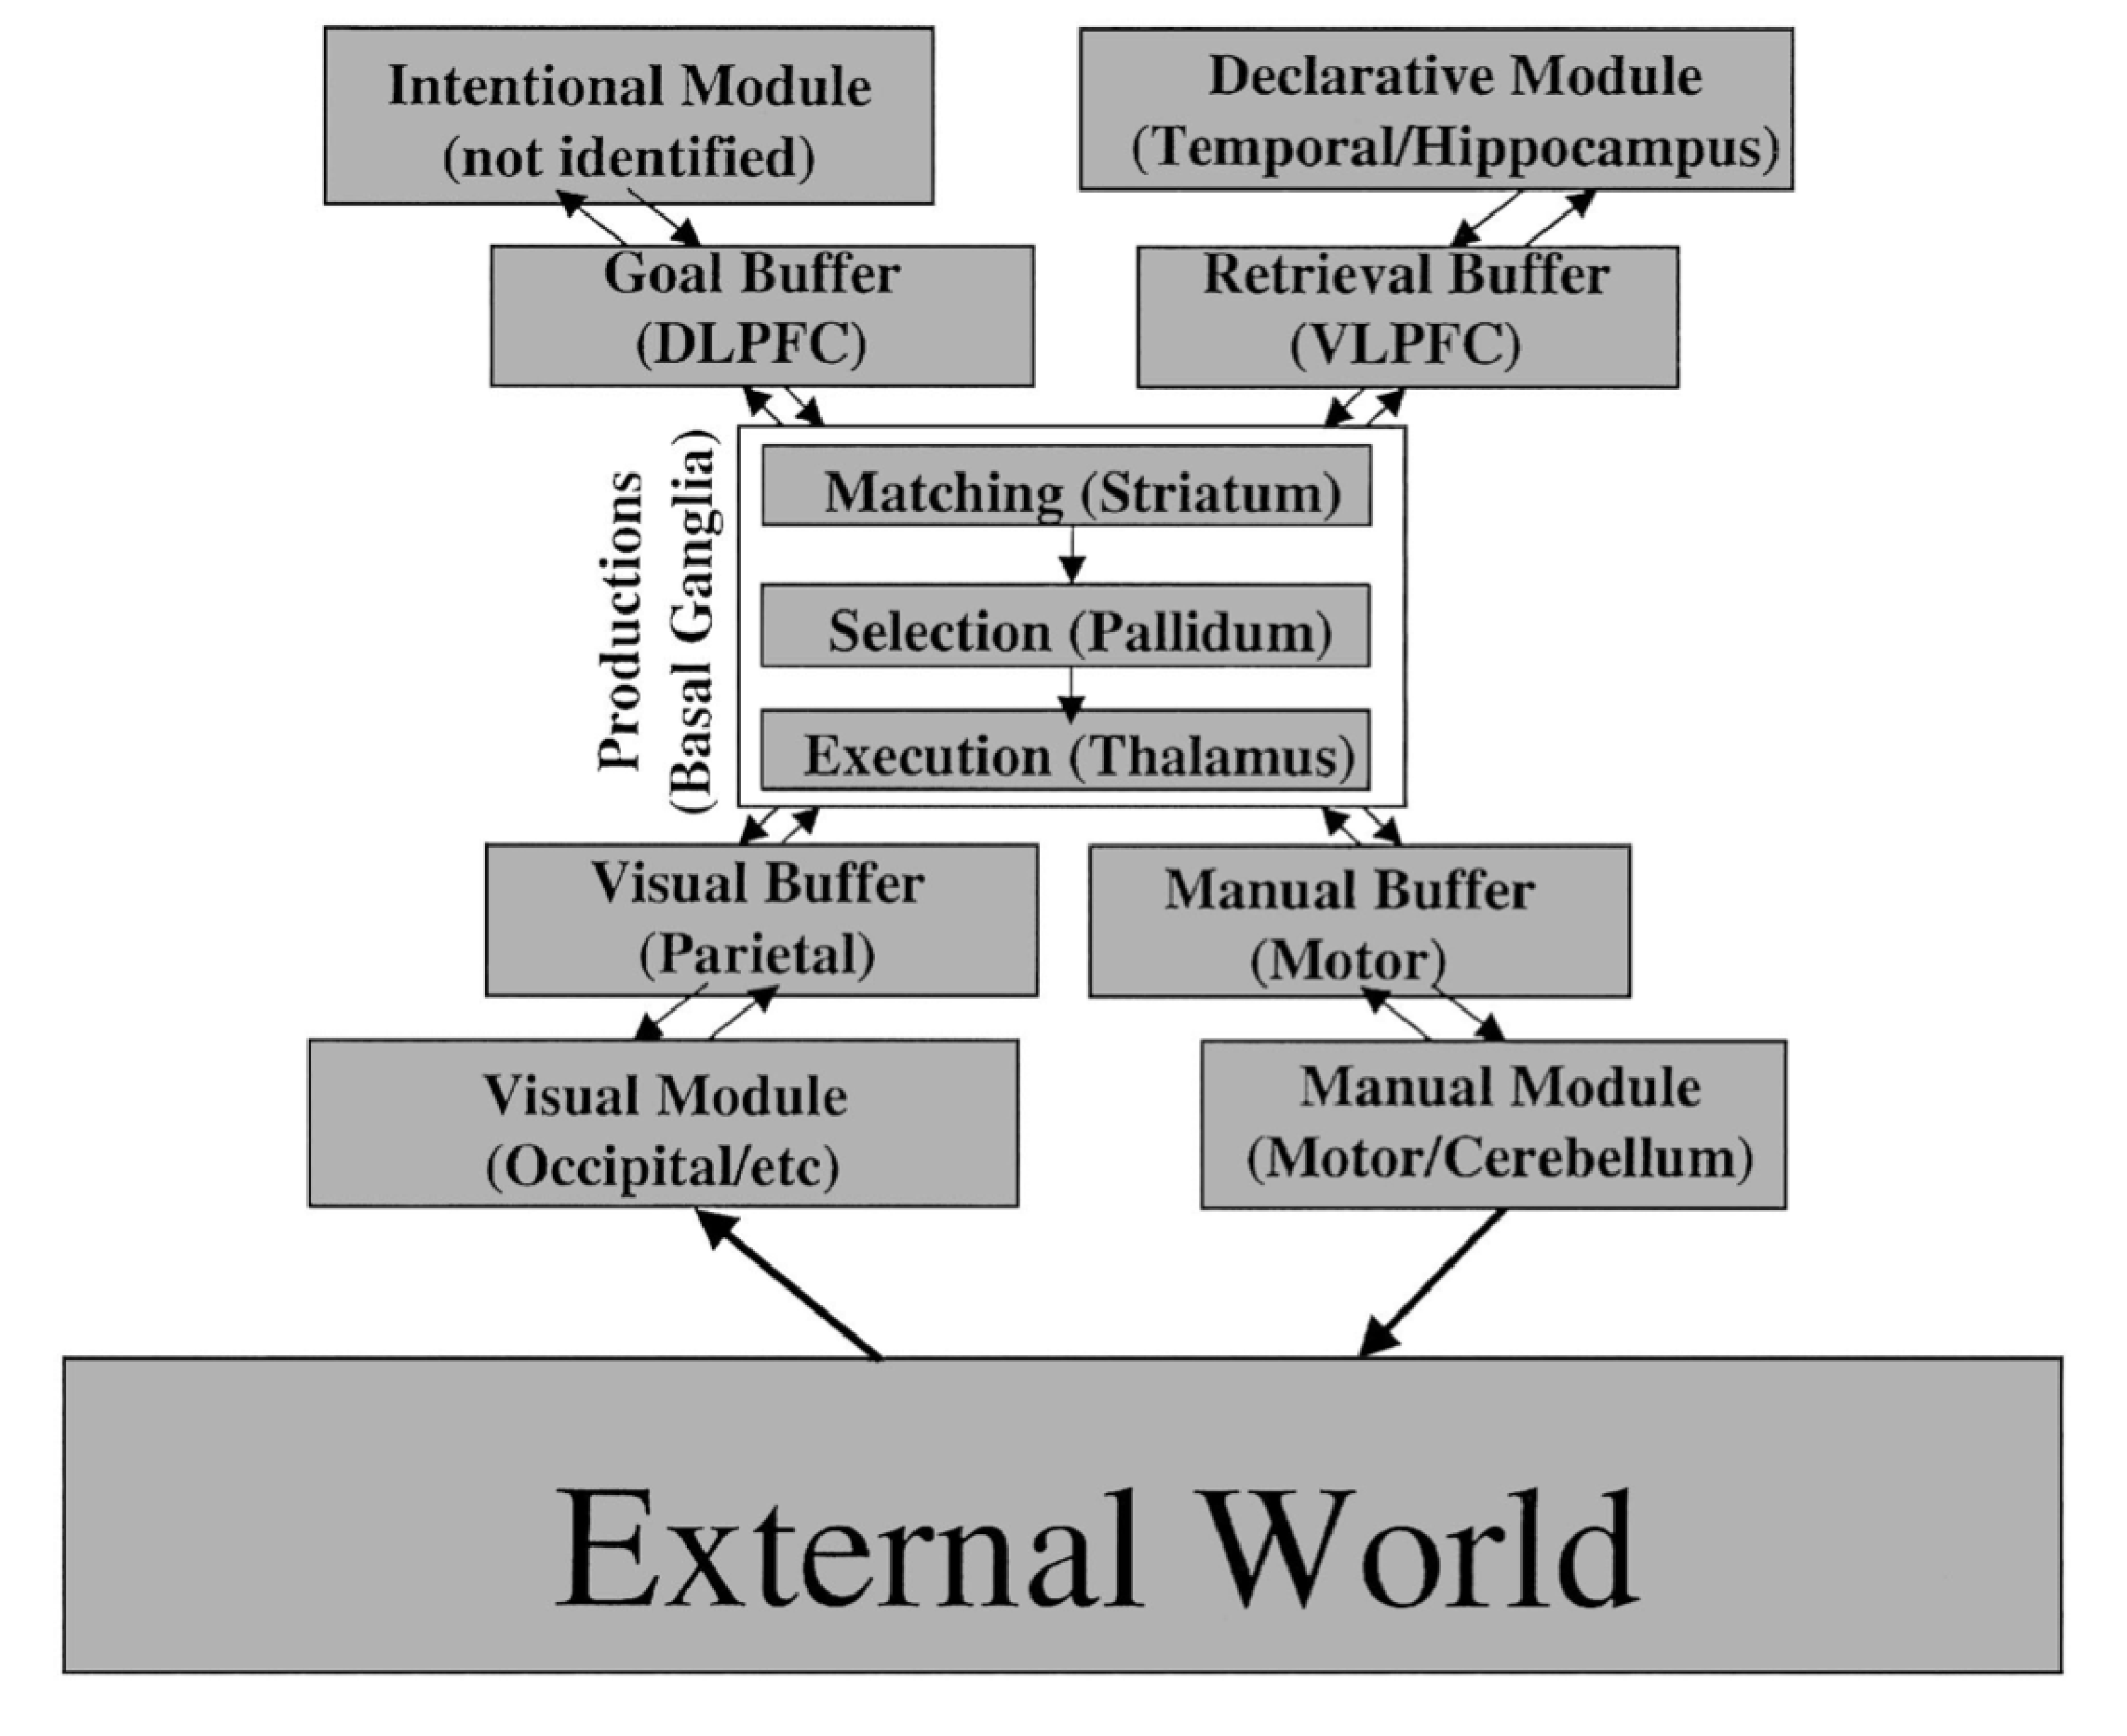
\includegraphics[width=100mm]{ACTRArch.eps}
  \caption{The architecture of ACT-R 5.0\cite{anderson_jr-etal:2004a}}
  \label{ACTR_ARCH}
\end{figure}


% Describe architecure

% Architecture Background
\actr was developed by Anderson et. al. \cite{anderson_jr-etal:2004a}
at Carnegie Mellon University to validate results performed by in the
area of cognitive psychology. \actr's origins lie in an attempt by
Anderson and Bower to describe a theory that explained the working of
memory called Human Associative Memory(HAM)\cite{AndersonBower73}. HAM
eventually grew into {\small ACT}\cite{Anderson76} which in due course evolved
into \actr\cite{Anderson83}.

% Describe the architecture given in the picture.
ACT-R consists of a set of core modules. These modules aim to
represent various constituent regions of the brain. The operation of
these modules is coordinated by a central production system. This
system can identify patterns and make changes to the contents of
buffers. The organization of these modules can be seen in figure
\ref{ACTR_ARCH}. I describe each of these modules below.

\begin{itemize}
\item {\bf Visual Module}: This module provides ACT-R with the capability of
  identifying objects visually.
\item {\bf Manual Module}: This module provides ACT-R with the ability to
  perform motor actions.
\item {\bf Intentional Module}: This module helps ACT-R simulate the
  ability to keep track of current goals.
\item {\bf Retrieval Module}: This module implements the mechanism to
  retrieve chunks of information from the declarative memory.
\end{itemize}

%   Knowledge representation, 
%      short term memory, long term memory, Goals,
In ACT-R information stored in human memory like phone numbers, words,
etc. are stored in chunks. Chunks can either be declared at the start
of the model or are created during the execution of the model. Chunks
represent information stored in the declarative memory. The
probability and the speed with which a chunk might be retrieved is
controlled by its activation. This is defined by the equation

\begin{equation}
  A_i = B_i + \sum_j W_j S_{ij}
\end{equation}

Where $A_i$: is the activation level of the chunk, $B_i$: is the base
level activation of the chunk, $W_j$ is the attentional weighting of
the elements of the current goal and $S_{ij}$ represents the strengths
of associations from elements j to chunk i.

%   Mechanics of cognition
%      Means of planning, Learning
The production system is the $<$CHOOSE WORD$>$ that controls the
coordination between various modules, this is done through selecting
the appropriate production and firing it. Though there may be a number
of competeing productions the one with the highest utility is
selected.  The utility of a production is defined by 

\begin{equation}
  U_i = P_iG - C_i
\end{equation}

where $P_i$ is the probability that the if production $i$ is selected
that the goal $G$ will be achieved. $C_i$ defines the cost to
completing the goal. This is estimated in the amount of time left to
complete the goal. 

ACT-R learns through a process of production compilation
\cite{oai:CiteSeerPSU:518586}. It attempts to teach successive pairs
of productions and tries to unify them into a single production. But
Anderson mentions that this breaks down when the productions consist
directives to the visual-motor modules.


%   Abilities of perception
%      Auditory, Visual, Motor
% The motor perceptual system
% The act-r motor perceptual system is essentially borrowed of the
% EPIC system.

The ACT-R motor-perceptual system is modeled after EPIC
(executive-process/interactive-control). The perception of vision is
provided by the visual module, which itself consists of two modules
the visual-location module and visual-object module. The
visual-location module helps the visual module to focus its attention
to a location in the visual field specified by the buffer. The
visual-object module holds information about the object in the visual
field. Motor control is provided by the manual module. ACT-R also has
rudimentary auditory and vocal modules\cite{anderson_jr-etal:2004a}.


% The approach taken was to model the basic timeing behaviour of those
% systems in an approximate form. The model the timing behaviour,
% input and output behaviours.

\subsection{SOAR}

% Describe architecture background
\soar is a general cognitive architecture proposed originally by Allen
Newell in \cite{Newell:1990aa,27702} when he argued for the need for
psychology to deal with human cognition as a whole, rather than in
form of micro strategies. The major ideas\cite{Lewis:2001aa} that
define the characteristics of \soar are:

% Describe the motivations behind SOAR, the technical ideas that
% constitute 
\begin{itemize}
\item \emph{Physical symbol systems}: \soar is a physical symbol
  system. Physical symbols systems are a class of system that are
  capable of manipulating symbols and according to the \emph{physical
    symbol system hypothesis}\cite{Newell1980135} are capable of
  demonstrating intelligent and flexible behavior.
\item \emph{Search in problem spaces}: \soar achieves cognition based
  on a \emph{search of problem spaces} and is supported by a
  \emph{recognize-decide-act} control structure. This is because
  Newell believed that human cognition was a result of a search of a
  problem space. This is known as the \emph{problem space
    hypothesis}\cite{162585}. 
\item \emph{Continuous, impasse driven learning}: \soar learns by
  a technique called \emph{chunking}. This topic is explained in
  detail below.


\end{itemize}

%   Knowledge representation, 
%      short term memory, long term memory, Goals,
According to the \soar theory human memory is composed to two separate
memories;long term memories, stores information for a long period of
time, and the working memory, stores information required for the task
currently at hand. 

Long term memory(LTM) stores information that is used to store
information that can be applied a number of instances of tasks. LTM is
composed of three memories: procedural memory, semantic memory and
episodic memory. Procedural memory stores information about how a task
is supposed to be carried out, for example it would store information
about task such as changing a light bulb, looking up a word in the
dictionary, etc. Semantic memory is used to store information related
to facts about the environment in which the agent operates, for
example in an environment where the agent is trying to replace a light
it would know that a light consists of a filament etc. Episodic memory
stores information about specific incidents along with contextual
information, $<$ \textsc{Think of a good example} $>$. Information
stored in the procedural memory is accessed more frequently than
information from either the semantic or episodic memories and this
information directly controls the behavior of the agent. 

All information in the LTM is stored in the form of
\emph{productions}. A production consists of a set of conditions and a
set of corresponding actions. Productions provide control information
for the application of operators on a candidate state in the Working
Memory. Productions perform four different roles: three knowledge
retrieval problem solving functions and a state elaboration
function. The knowledge retrieval functions are operator proposal,
operator comparison and operator
application\cite{Laird:2006aa}. Productions in \soar are fired in
parallel with out conflict resolution unlike \actr that has a conflict
resolution mechanism to select between competing productions.

\emph{Preference Memory} is used to decide which operator is the best in the
given circumstance.  Preferences in the memory are used to compare a
selected set of operators with one another in an attempt to pick up
the best operator. Actions in productions are instrumental in creating
productions. These remain active as long as the production is deem
suitable for the situtation and are removes once the production is not
valid.

\emph{Working Memory}(WM) describes memory that hold information
related to the task that is currently being executed. This includes
states and sub-states created to solve the problem, operators that are
applicable to the current states and Working memory elements(WME) that
hold specific information about a specific identifier. Elements in the
working memory are created by the action of productions, a state
created as a result of an \emph{impasse}, $<$ ASK FOR EXPLANATION
POINT three from paper $>$ or because of the action of external IO
systems. Information from the working memory is removed only when it
becomes irrelevant to the existing situtation. This architecture can
be seen in figure \ref{SOAR_ARCH}.

\begin{figure}[htp]
  \centering
  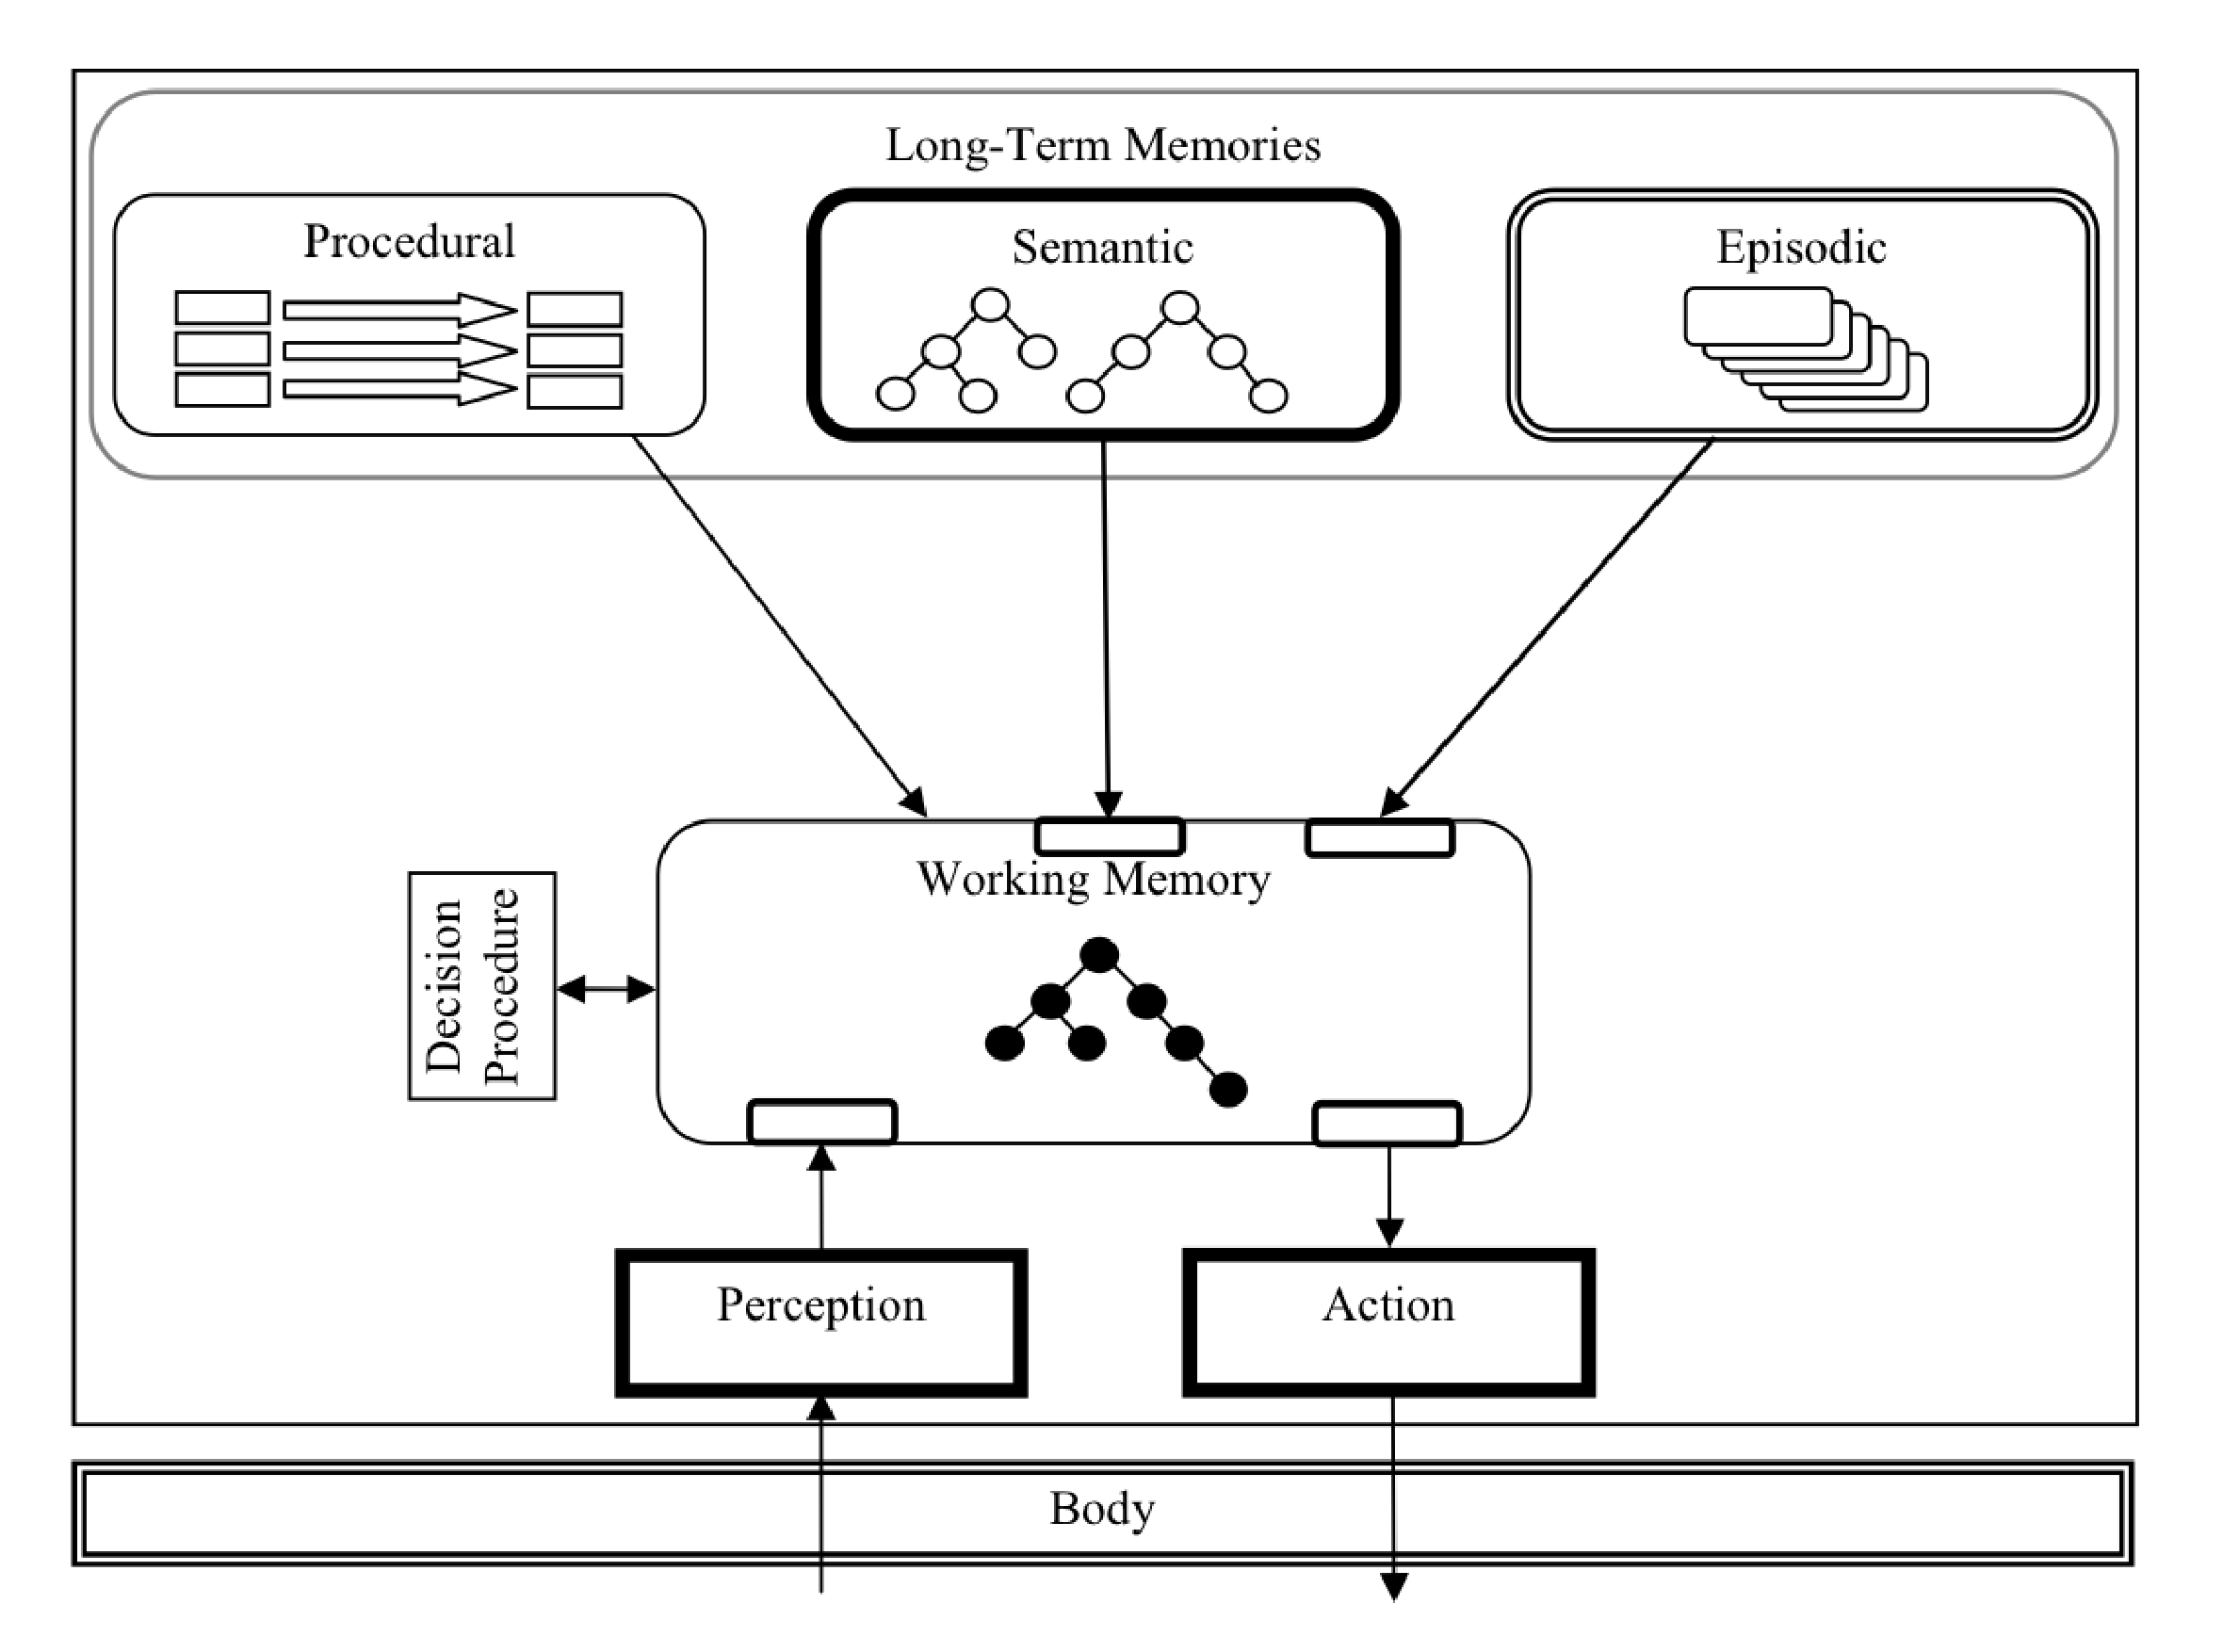
\includegraphics[width=100mm]{soar.eps}
  \caption{Soar Architecture\cite{Jill-Fain-Lehman:2006aa}}
  \label{SOAR_ARCH}
\end{figure}

%   Mechanics of cognition
%      Means of planning, Learning
% Describe searching in a space, impasses, subgoaling, creation of new states
\soar believes that cognition is flexible and goal driven, learning
is a continuous experience that arises from experience. 
% Give an overview of chunking
 
%   Abilities of perception
%      Auditory, Visual
$<$ \textsc{The \soar architecture does not describe its perceptual
  motor facilities in detail. What do I write about that?} $>$
% Give a general over view of the input and output capabilities

\subsection{EPIC}
\subsection{CLARION}
\subsection{Subsumption Architecture}

\subsection{Criteria for comparison}



% Things to be concerned about
% 1) Perception: How an architecture gets its input
% 2) Memory: How is memory represented
% 3) Goals: How goals are represented and solved
% 4) Problem Solving: Techniques for solving problems
% 5) Planning: Planning techniques used 
% 6) Reasoning: How do system reason
% 7) Learning: How stuff is learnedn
% 8) Meta Processing: ??
% 9) Natural language processing: How is natural language processed
% 10) Query Answering: Not required
% 11) Diagnosis: Not required
% 15) Ability to recover from failure
% 18) Reusability
% 19) Mapping to the brain


% Architectures to compare

% CLARION
% SOAR
% EPIC
% ACT-R
% Subsumption
\section{Challenges facing cognitive architectures}

%Summarise this section
This section attempts to provide a brief a explanation to the nature
of human cognition. It also surveys a number of cognitive
architectures and attempts to provide a brief overview of the state of
the art in the area of cognitive architectures. 


% Say though all this work there are still some open issues, cite the
% paper and describe the issues.
Despite the tremendous amount of effort that has gone in this area, we
are no where near the end. There are a number of research questions
that are open for curious minds to explore. These areas are spelled
out very clearly by Langley et. al. in \cite{citeulike:4182324}


\begin{itemize}
\item \emph{Architectures need to explore categorization and
    understanding}: Currently cognitive architectures have not paid
  significant attention to the means by which we understand concepts
  and ideas. It also the case with categorization. Categorization is
  the ability of humans to categorize object that may seem dissimilar
  at first. 
  
\item \emph{Accurately reflecting perceptive abilities of physical
    agents}: Most architectures tend to ignore the fact that a human
  has limited abilities to focus on any task. Architectures need to
  replicate this behaviour if we are to acquire a greater
  understanding of human cognition.

% People Need to focus more on episodic knowledge
  \item \emph{Further emphasis on episodic memory}: Episodic memory is
    a form of declarative memory that also requires context and also
    personal participation\cite{09011999}, for example, a person's
    eighteenth birthday.  Focus on problem solving and skills has
    distracted the cognitive architecture community from studing the
    complete nature of episodic memory.

% Extend frameworks to build knowledge formalisms to enable
% intelligent behaviour
\item \emph{Further study of knowledge representation}: Humans use a
  number of ways of representing knowledge using visual or auditory
  representations unlike most cognitive architectures that have
  essentially been tied down to representing knowledge in the form of
  production rules or similar forms. There has to be a further study
  in various representational schemes that can be used such as
  frames\cite{Minsky1974a} and description logics
  \cite{nardi-brachman:2003a}. 
%\textsc{REUBEN:TODO:get a background    on description logics}

% No cognitive architectures handle interaction between body and mind.
\item \emph{Study of body-mind interaction}: Despite the large number
  of topics addressed in cognitive architecture reseach, the area of
  body-mind interaction has not been explored in detail.

% Emotions, no architectures handle that

\item \emph{Study of emotion}: Emotions is what defines humans and in
  quite a few cases control their actions. In quite a few instances
  emotions determine the actions of humans. The area of cognitive
  science and cognitive architectures needs to explore would need to
  explore this area to get a more complete picture of human cognition.

% use natural language processing more
% \item \emph{Farther the use of natural language:} Cognitive
%   architectures have done a considerab
% This point does not hold, because I would rather have raw data on
% which I would be able to run a whole lot of metrics rather than
% having any other sort of output.
% REUBEN:TODO:Speak to prof about this.


\end{itemize}

%This is more of an engineering point of view, the idea is that most
%cognitive architectures do not support reuse as a part of the
%them. This project is a step in exploring how models can be shared
%and reused.

% from an engineering stand point if it would ease development if we
% re use would help ease of development 

From an engineering standpoint a cognitive modeller essentially
building intelligent agents and in quite a number of cases work done
by one researcher can be reused elsewhere by someone else. The
advantages of providing such a system would be

% Quicker development times
% Lesser bugs
% Greater coherence
% Areas can be explored more thoroughly because creating models is
% easy and cheap
% Sharing knowledge and resources

As far as e know no one has attempted to solve this problem. No of
cognitive architectures and the aim of this project is to take a step
in that direction.


\textsc{TODO: Mention converging trends in research: Merge stuff from
  the Chong and David Vernon paper}